\documentclass{article}

% if you need to pass options to natbib, use, e.g.:
% \PassOptionsToPackage{numbers, compress}{natbib}
% before loading nips_2016
%
% to avoid loading the natbib package, add option nonatbib:
% \usepackage[nonatbib]{nips_2016}

%\usepackage{nips_2016}

% to compile a camera-ready version, add the [final] option, e.g.:
\usepackage[final]{nips_2016}

\usepackage[utf8]{inputenc} % allow utf-8 input
\usepackage[T1]{fontenc}    % use 8-bit T1 fonts
\usepackage{hyperref}       % hyperlinks
\usepackage{url}            % simple URL typesetting
\usepackage{booktabs}       % professional-quality tables
\usepackage{amsfonts}       % blackboard math symbols
\usepackage{nicefrac}       % compact symbols for 1/2, etc.
\usepackage{microtype}      % microtypography
%\usepackage{amssymb}
%\usepackage{color}
%\usepackage{amsthm}
%\usepackage{amsmath}
%\usepackage{indentfirst}
\usepackage{tcolorbox}
\usepackage[ruled]{algorithm2e}
%\usepackage{apacite}
%\usepackage{graphicx}
\usepackage{subcaption}

\newtheorem{theorem}{Theorem}
\newtheorem{lemma}{Lemma}
\newtheorem{definition}{Definition}

\title{Robust Single Linkage Algorithm and Extract Flat Clustering}

% The \author macro works with any number of authors. There are two
% commands used to separate the names and addresses of multiple
% authors: \And and \AND.
%
% Using \And between authors leaves it to LaTeX to determine where to
% break the lines. Using \AND forces a line break at that point. So,
% if LaTeX puts 3 of 4 authors names on the first line, and the last
% on the second line, try using \AND instead of \And before the third
% author name.

\author{
  Taoran Xue \\
  Department of Computer Science\\
  George Washington University\\
  Washington, DC 20052 \\
  \texttt{taoran\_xue@gwu.edu} \\
  %% examples of more authors
  %% \And
  %% Coauthor \\
  %% Affiliation \\
  %% Address \\
  %% \texttt{email} \\
  %% \AND
  %% Coauthor \\
  %% Affiliation \\
  %% Address \\
  %% \texttt{email} \\
  %% \And
  %% Coauthor \\
  %% Affiliation \\
  %% Address \\
  %% \texttt{email} \\
  %% \And
  %% Coauthor \\
  %% Affiliation \\
  %% Address \\
  %% \texttt{email} \\
}

\begin{document}
	
	\maketitle
	
	\section{Instruction}
	
	In unsupervised learning algorithm, there exists two problem to solve. First is that if our data set is infinity, in another word, its size can be increasing in a time, we need a cluster algorithm to fit the distribution density function of the data set. Second, if some bad or noise point occasionally draws between two cluster, it will influence the cluster result different from the original distribution of probability density function.
	
	\section{Minimum spanning tree}
	
	Before we go through today's topic, let's have a quick review of my last presentation about density based hierarchy clustering algorithm. Because we are trying to give a robust single linkage algorithm based on previous method.
	
	
	
		For each $i$, set $r(x_i)$ to the distance from $x_i$ to its $k$th nearest neighbor.
		
		As $r$ grows from $0$ to $\infty$:
		\begin{enumerate}
			\item Construct a graph $G_r$ with nodes $\{x_i : r(x_i) \leq r\}$. Include edge $(x_i, x_j)$ if $\|x_i - x_j\| \leq$ $\alpha r$.
			\item Let $\mathbb{C}_n(r)$ be the connected components of $G_r$.
		\end{enumerate}  
		
	
	As we know, real data is messy and has corrupt data, and noise. So we need to make a new algorithm with single linkage algorithm and it can be sensitive to noise. As I mentioned, if a single noise data point is in the wrong place can act as a ``thin bridge'' between two cluster, gluing them together.
	
	\begin{figure}[h!]
		\centering
		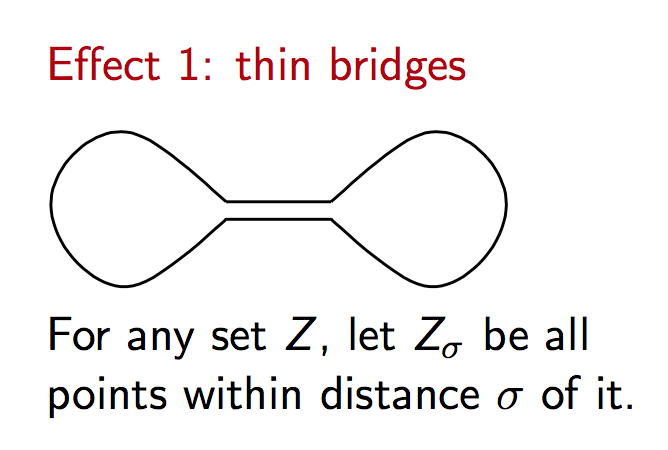
\includegraphics[scale=0.35]{a.png}
		\caption{``Thin bridge'' effect.}
		\label{fig:slabfig}
	\end{figure}
	
	So the authors of previous paper[2] give a method to robustly process against noise, and, in the paper presentation, I proved that this algorithm can deal with noise problem. Their idea is to define a new version of minimal spanning tree.
	
		\begin{definition}
			Set $r_k(x_i)$ to the distance to $k$th nearest neighbor. For any $r = \mathrm{max}\{r_k(x_i)\}$, connect points $x_i$ and $x_j$, if $||x_i - x_j|| \leq \alpha r$.
		\end{definition}
	
	Thus, [1] convert it to our new definition mutual reachability distance:
	
		\begin{definition}
			Set $core_k(x_i)$ to the distance to $k$th nearest neighbor.
			$$d_{\mathrm{mrd}_k}(x_i, x_j) = \mathrm{max}\{core_k(x_i), core_k(x_j), ||x_i - x_j||\}$$
		\end{definition}
	
	As we have mutual reachability distance matrix, we can build the minimum spanning tree very efficiently via Prim's algorithm.
	
%\begin{comment}
	\begin{figure}[h!]
		\begin{subfigure}{.5\textwidth}
			\centering
			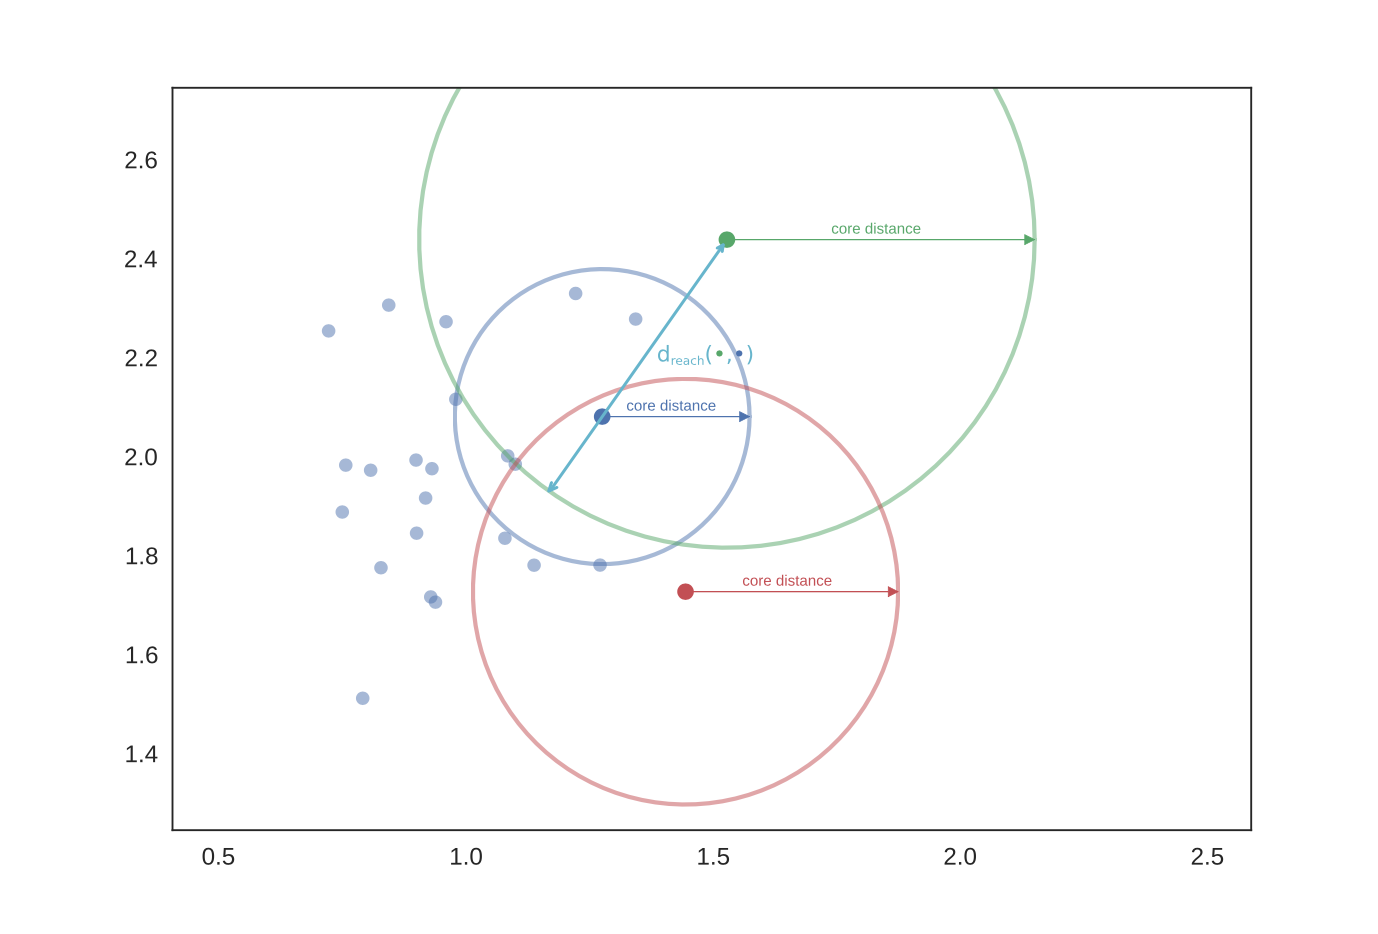
\includegraphics[width=\linewidth]{dis_figure1.png}
			\caption{}
		\end{subfigure}%
		\begin{subfigure}{.5\textwidth}
			\centering
			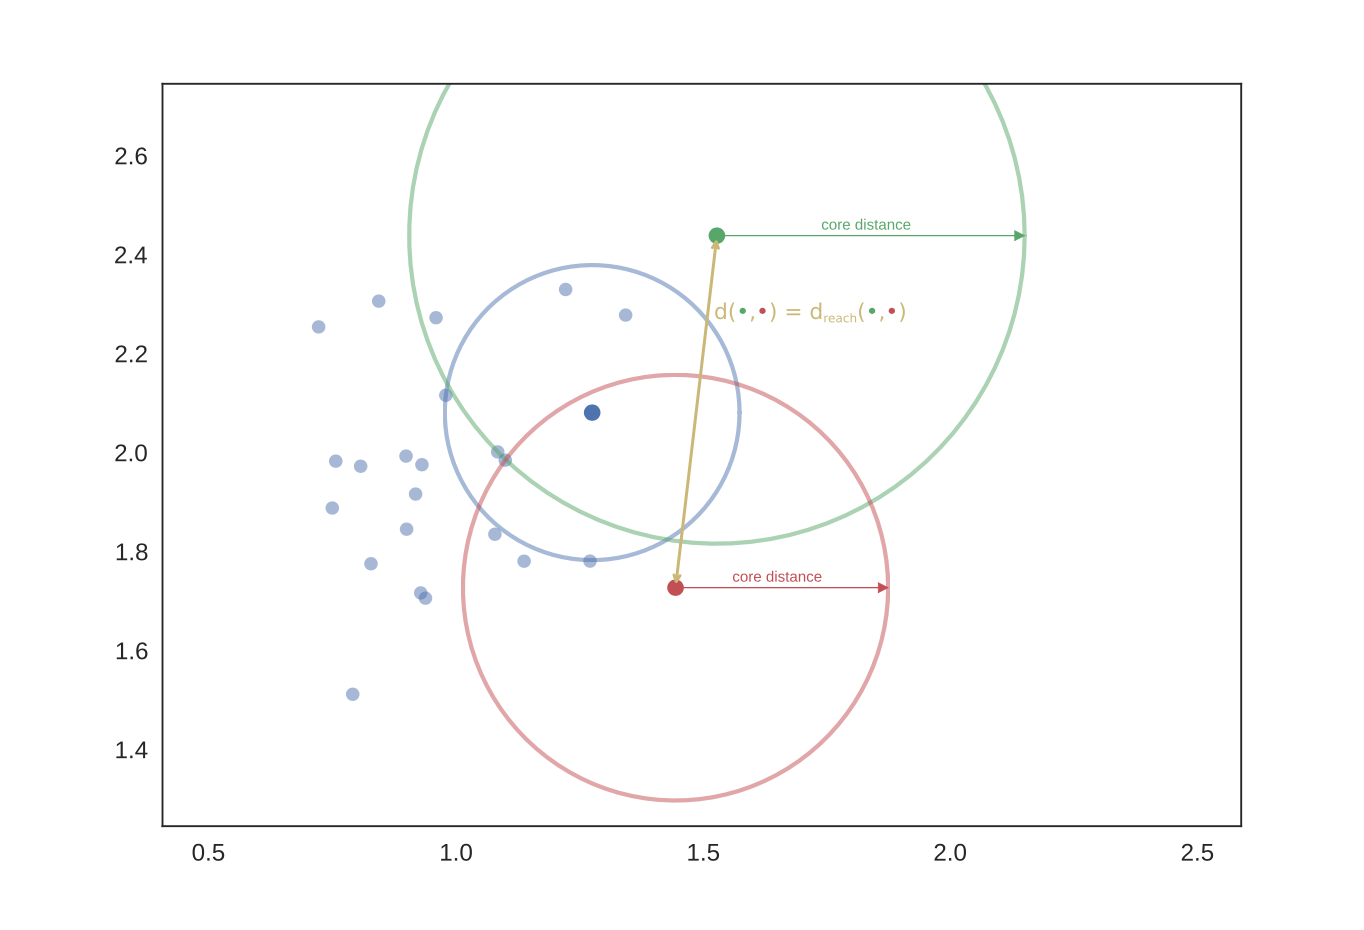
\includegraphics[width=\linewidth]{dis_figure2.png}
			\caption{}
		\end{subfigure}
		\caption{Mutual reachability distance}
	\end{figure}
%\end{comment}
	
	\section{Single linkage hierarchy algorithm}
	
	Given the minimal spanning tree, the next step is to convert that into the hierarchy of connected components. This is most easily done in the reverse order: sort the edges of the tree by distance (in increasing order) and then iterate through, creating a new merged cluster for each edge. 
	
	\section{Condense tree}
	
	Hierarchy cluster algorithm always gets a large and complicated cluster hierarchy tree. So [3] try to condense down the cluster hierarchy into a smaller tree. In another word, we are trying to make cluster tree pruning to get a simpler cluster tree. As you can see in the hierarchy above it is often a cluster split is one or two points splitting off from a cluster. We need to eliminate cluster which has fewer points than the minimum cluster size. 
	
	Initially, we breadth-first search the whole hierarchy tree. When we arrive one cluster, there will be three conditions.
	
	\begin{itemize}
		\item If left child cluster point number is greater than minimum cluster size, but right side is not, Figure \ref{fig:condtree} (a), keep the left branch and ignore right cluster;
		\item If left and right child clusters are both greater than minimum cluster size, Figure \ref{fig:condtree} (b), we consider that a cluster split and let the split persist the whole tree;
		\item If left and right child clusters are both fewer than minimum cluster size, Figure \ref{fig:condtree} (c), we ignore the two cluster.
	\end{itemize}
	
	\begin{figure}[h!]
		\centering
		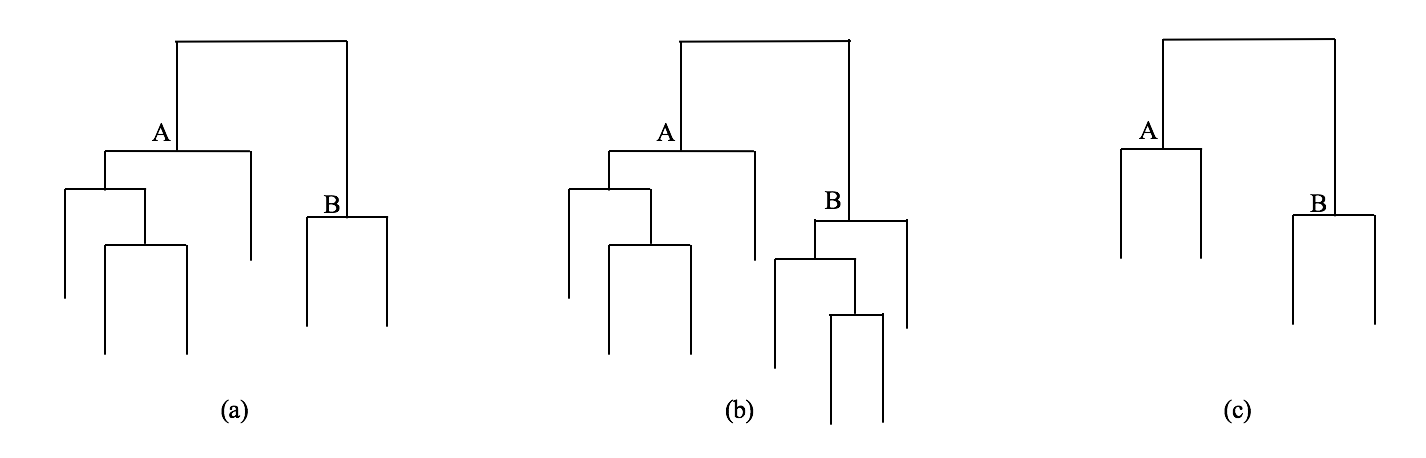
\includegraphics[scale=0.45]{b.png}
		\caption{Condense tree pruning method .}
		\label{fig:condtree}
	\end{figure}
	
	\begin{algorithm}[H]
		\SetAlgoNoLine
		\SetKwData{minClusterSize}{minClusterSize}
		\SetKwData{numPoints}{numPoints}
		\SetKwData{left}{left}
		\SetKwData{leftCount}{leftCount}
		\SetKwData{right}{right}
		\SetKwData{rightCount}{rightCount}
		\SetKwData{p}{p}
		\SetKwData{tmpNode}{tmpNode}
		\SetKwArray{nodeList}{nodeList}
		\SetKwArray{H}{H}
		\SetKwArray{T}{T}
		\SetKwArray{nextLabel}{nextLabel}
		\SetKwFunction{BFS}{BFS}
		\KwIn{\H{$m$} $\leftarrow$ hierarchy tree contains a tuple of (child1,child2,distance,childrenSize), \minClusterSize $\leftarrow$ The minimum size of clusters to consider}
		\KwOut{\T{$n$} $\leftarrow$ condense tree contains a tuple of (parent,child,$\lambda$,childrenSize)}
		\nodeList $\leftarrow$ \BFS{$H$}\;
		\For{$r \leftarrow 0$ \KwTo $m$}{
			\If{\nodeList{r} is ignored} {Pass\;}
			\left $\leftarrow$ \nodeList{r}.child1\;
			\leftCount  $\leftarrow$ \H{\left}.childrenSize\;
			\right $\leftarrow$ \nodeList{r}.child2\;
			\rightCount  $\leftarrow$ \H{\right}.childrenSize\;
			\If{\leftCount $\geq$ \minClusterSize \textbf{and} \rightCount $\geq$ \minClusterSize}{
				\T{{\p}$++$} $\leftarrow$ (\nextLabel, $++${\nextLabel}, $1/\mathrm{distance}$, \leftCount)\;
				\T{{\p}$++$} $\leftarrow$ (\nextLabel, $++${\nextLabel}, $1/\mathrm{distance}$, \rightCount)\;
			}
			\If{\leftCount $<$ \minClusterSize}{
				\For{\tmpNode \textbf{in} \BFS{\left}}{
					\If{\tmpNode is leaf}{
						\T{{\p}$++$} $\leftarrow$ (\nextLabel, \tmpNode, $1/\mathrm{distance}$, $1$)\;
					}
					Ignore \tmpNode\;
				}
			}
			\If{\rightCount $<$ \minClusterSize}{
				\For{\tmpNode \textbf{in} \BFS{\right}}{
					\If{\tmpNode is leaf}{
						\T{{\p}$++$} $\leftarrow$ (\nextLabel, \tmpNode, $1/\mathrm{distance}$, $1$)\;
					}
					Ignore \tmpNode\;
				}
			}
		}
		\caption{Condense hierarchy cluster tree}
	\end{algorithm}
	
	
	\section{Cluster stability}
	
	For a condense tree, intuitively, we want to extract the cluster that persists and has a long lifetime. It means the cluster is relatively stable unlikely to split into two clusters after it created. So we give a new definition to measure the persistence of a cluster.
	
		\begin{definition}
			Let $\lambda = \frac{1}{d_{\mathrm{mrd}_k}}$. For each cluster we give $\lambda_{\mathrm{birth}}$ and $\lambda_p$ to be the lambda value when the cluster split off then became it’s own cluster, and the lambda value (if any) when the cluster split into smaller clusters respectively.
		\end{definition}
	
	Now, for each cluster $C$ compute the stability to as:
	
	$$ S(C) = \sum_{p \in {C}} (\lambda_p - \lambda_{\mathrm{birth}})$$
	
	\begin{algorithm}[H]
		\SetAlgoNoLine
		\SetKwArray{birthLambda}{birth$\lambda$}
		\SetKwData{currChild}{currChild}
		\SetKwData{prevChild}{prevChild}
		\SetKwData{currLambda}{curr$\lambda$}
		\SetKwData{minLambda}{min$\lambda$}
		\SetKwFunction{Min}{Min}
		\SetKwArray{T}{T}
		\SetKwArray{S}{S}
		\KwIn{\T{$n$} $\leftarrow$ condense tree in reverse topological order contains a tuple of (parent,child,$\lambda$,childrenSize)}
		\KwOut{\S{$n$} $\leftarrow$  stability of every node in condense tree}
		\For{$r \leftarrow 0$ \KwTo $n$}{
			\currChild $\leftarrow$ \T{$r$}.child\;
			\currLambda $\leftarrow$ \T{$r$}.$\lambda$\;
			\eIf{\currChild $=$ \prevChild}{
				\minLambda $\leftarrow$ \Min{\minLambda, \currLambda}\;
			}{
				\birthLambda{\currChild} $\leftarrow$ \minLambda\;
				\prevChild $\leftarrow$ \currChild\;
				\minLambda $\leftarrow$ \currLambda\;
			}
		}
		\For{$r \leftarrow 0$ \KwTo $n$}{
			$\S{r} \leftarrow \S{r} + \T{r}.\lambda - $\birthLambda{\T{r}.$\mathrm{parent}$} $\times \T{r}. \mathrm{childrenSize}$ \;
		}
		\caption{Calculate stability of each cluster}
	\end{algorithm}
	
	\section{Flat clustering}
	
	To make hierarchy cluster result to flat cluster result, we require that once the cluster is selected, then the descendant of it cannot be selected. Because hierarchy cluster is nested, selected cluster contains all cluster of its descendant.
	
		\begin{definition}
			Set $SC(C)$ is the sum of the stabilities of the child cluster of cluster $C$.
			$$SC(C) = \sum_{q \in C}S(c)$$
		\end{definition}
	
	\begin{algorithm}[H]
		\SetAlgoNoLine
		\SetKwData{subtreeStabilities}{subtreeStabilities}
		\SetKwData{childList}{childList}
		\SetKwData{tmpNode}{tmpNode}
		\SetKwFunction{Bfs}{Bfs}
		\SetKwArray{S}{S}
		\SetKwArray{L}{L}
		\KwIn{\S{$n$} $\leftarrow$  stability of every node in condense tree sorted in reverse topological order}
		\KwOut{\L{$n$} $\leftarrow$ \textbf{True} if index of cluster is selected; \textbf{False} otherwise}
		\L $\leftarrow$ \{\textbf{True}\}\;
		\For{$r \leftarrow 0$ \KwTo $n$}{
			\childList $\leftarrow$ \{list of node whose parent is $r$\}\;
			\subtreeStabilities $\leftarrow$ $\sum_{c \in \childList} \S{c}$\;
			\eIf{\subtreeStabilities $>$ \S{$r$}}{
				\L{$r$} $\leftarrow$ \textbf{False}\;
				\S{$r$} $\leftarrow$ \subtreeStabilities\;
			}{
				\For{\tmpNode \textbf{in} \BFS{$r$}}{
					\If{\tmpNode $\neq r$}{\L{\tmpNode} $\leftarrow$ \textbf{False}}
				}
			}
		}
		\caption{Abstract cluster with stabilities}
	\end{algorithm}
	
	\section{Experiment}
	
	This experiment aims at showing characteristics of this clustering algorithms on datasets that are ``interesting'' but still in 2D. The last dataset is an example of a ``null’' situation for clustering.
%\begin{comment}
	
	\begin{figure}[h!]
		\begin{subfigure}{.5\textwidth}
			\centering
			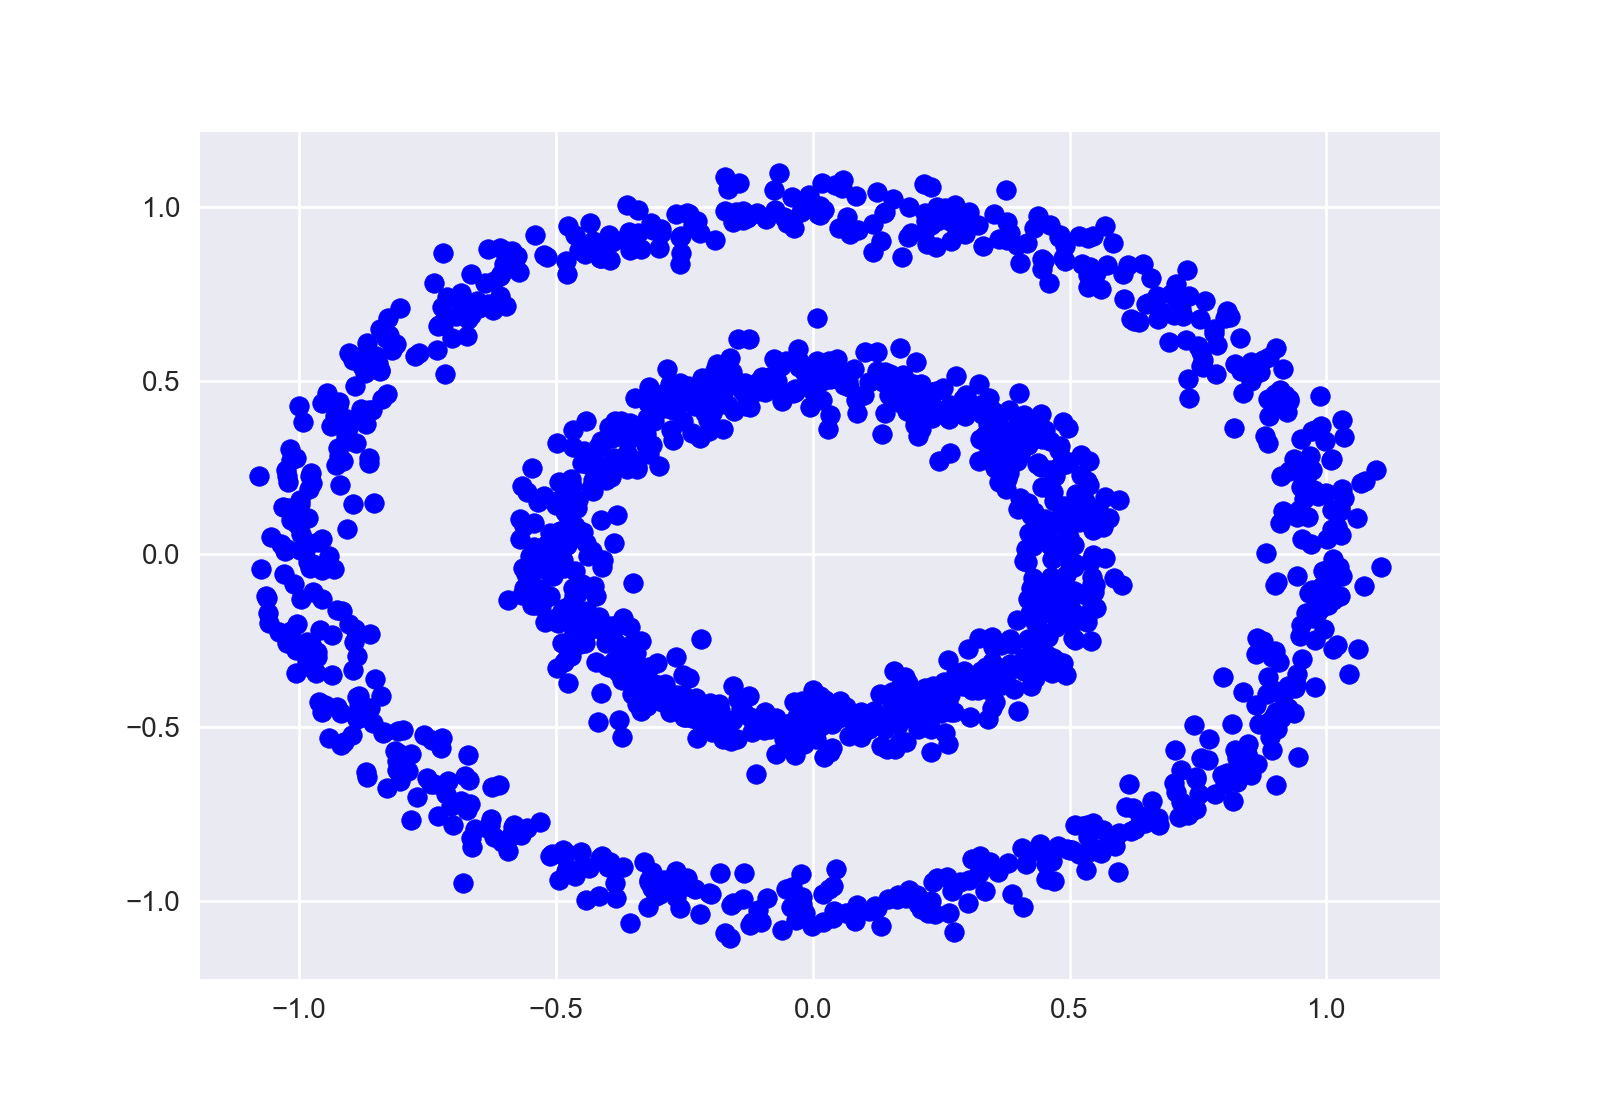
\includegraphics[width=\linewidth]{c_figure_1.png}
			\caption{}
		\end{subfigure}%
		\begin{subfigure}{.5\textwidth}
			\centering
			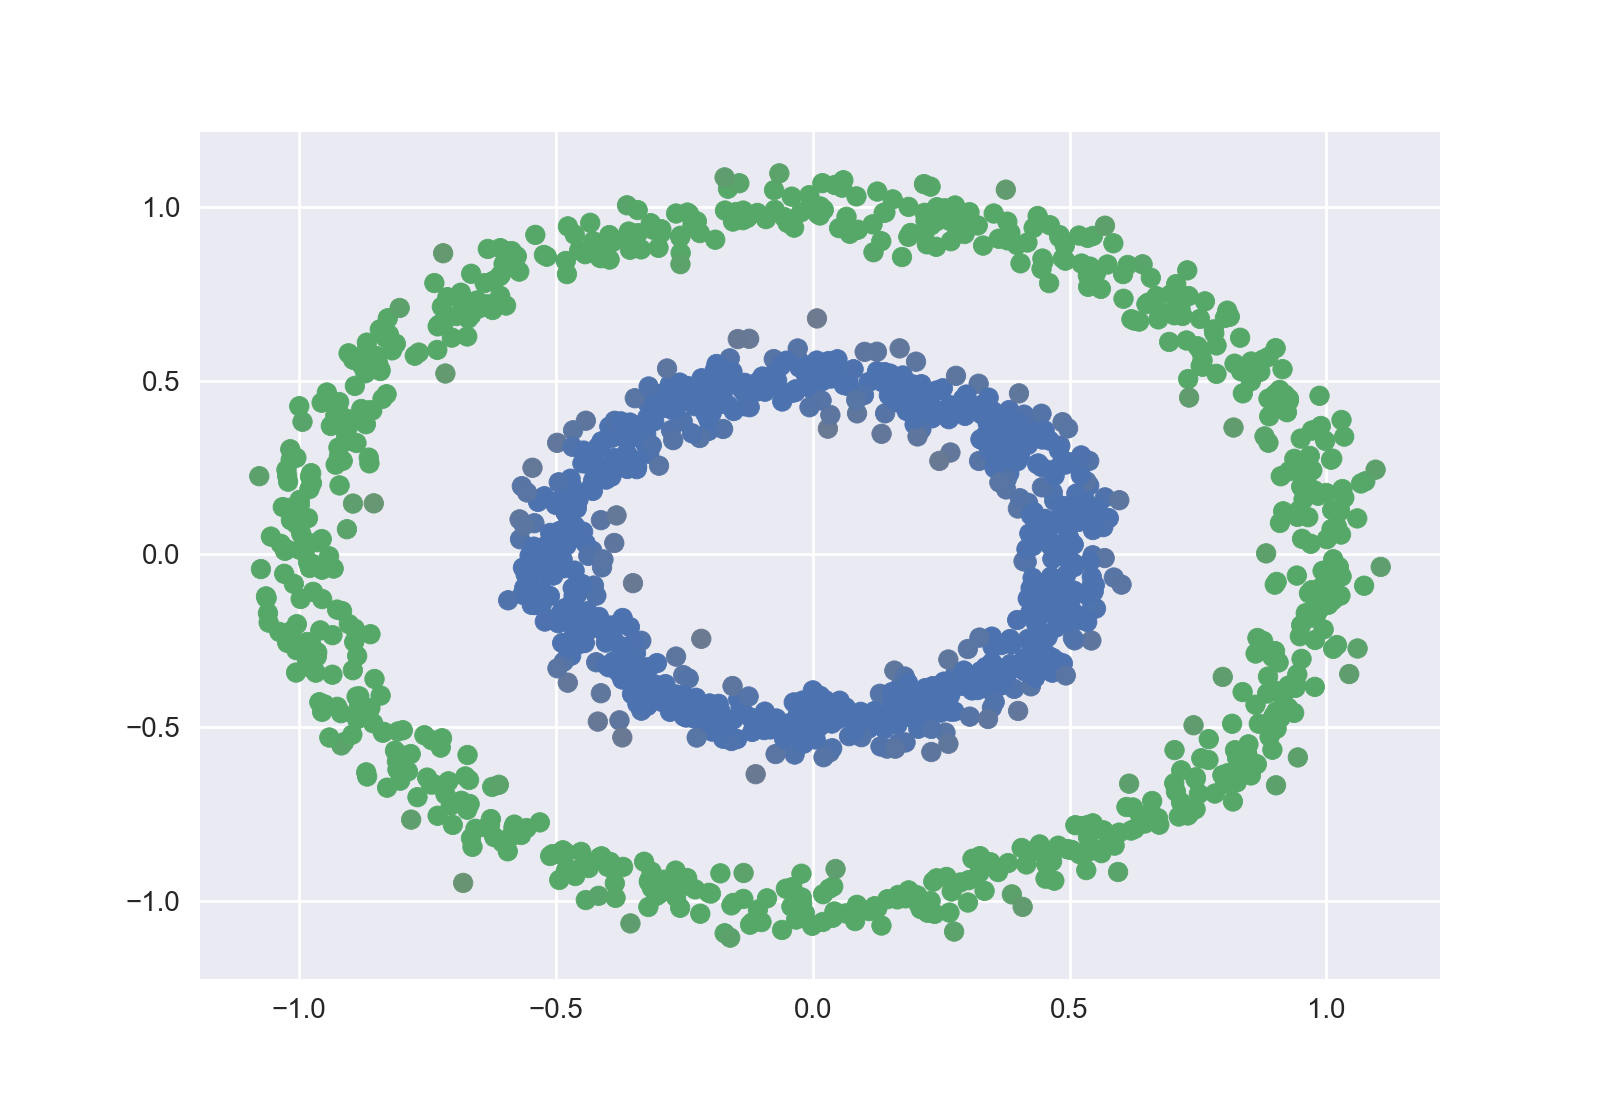
\includegraphics[width=\linewidth]{c_figure_2.png}
			\caption{}
		\end{subfigure}
		\caption{Clusters of circles}
	\end{figure}
	
	\begin{figure}[h!]
		\begin{subfigure}{.5\textwidth}
			\centering
			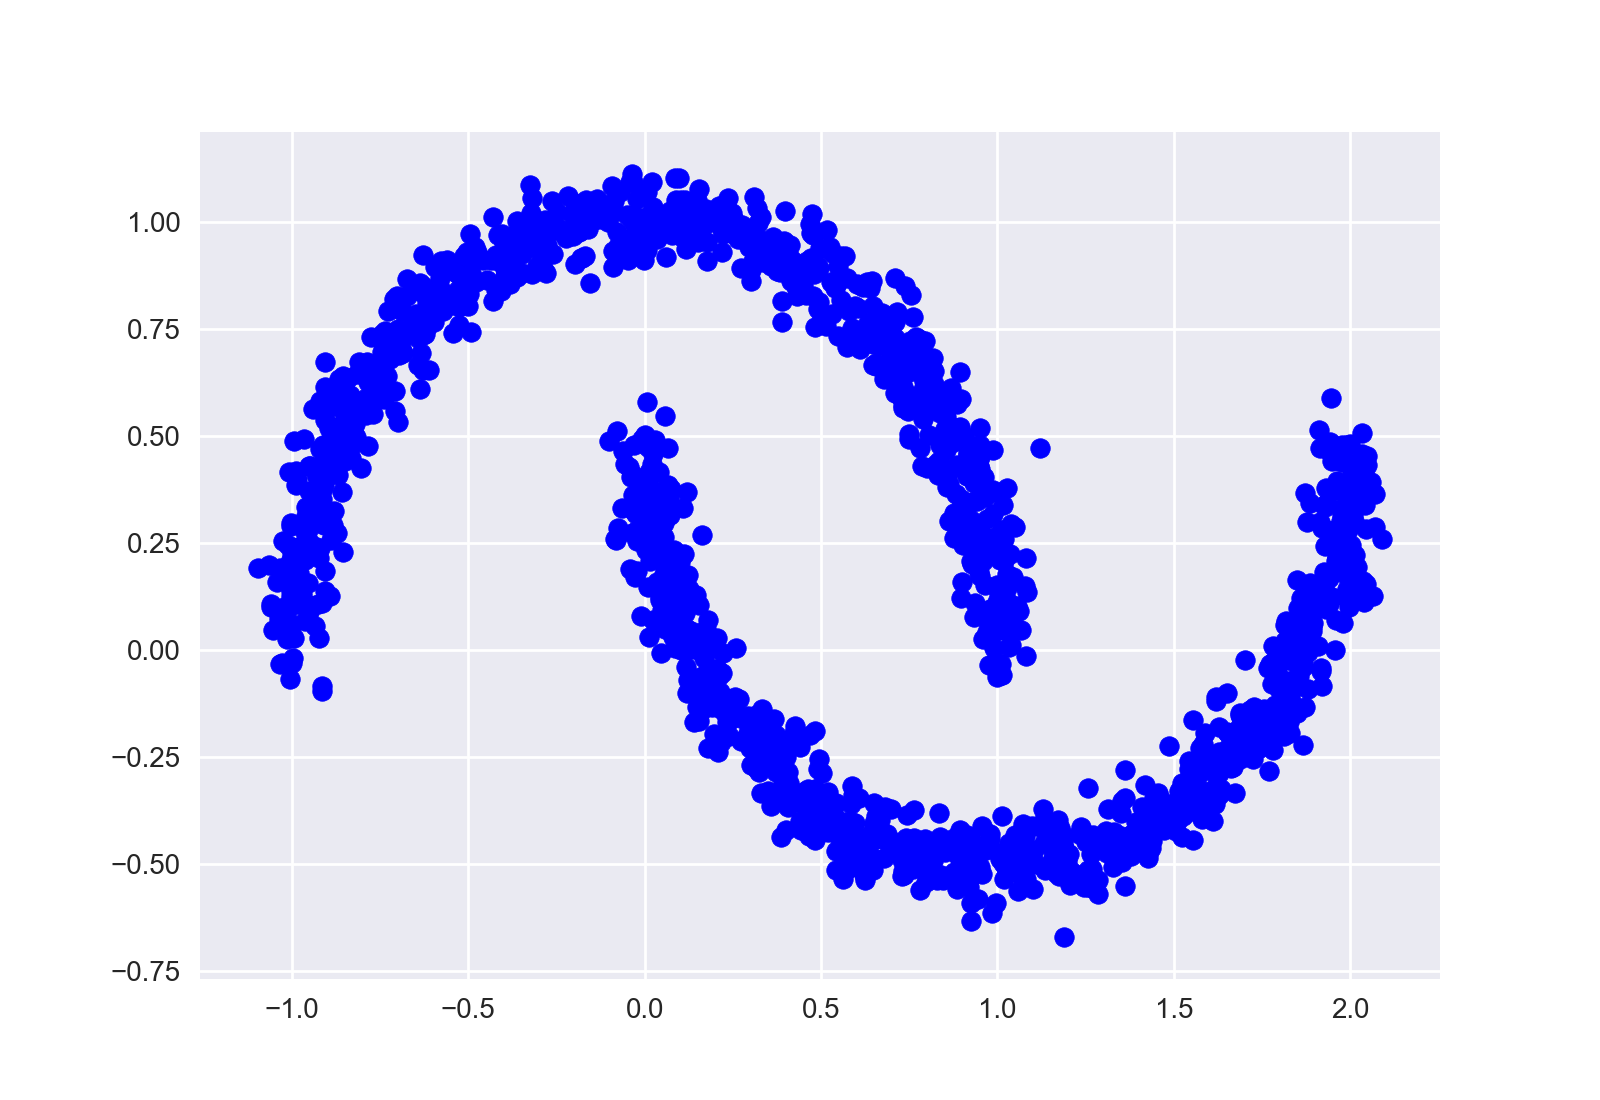
\includegraphics[width=\linewidth]{m_figure_1.png}
			\caption{}
		\end{subfigure}%
		\begin{subfigure}{.5\textwidth}
			\centering
			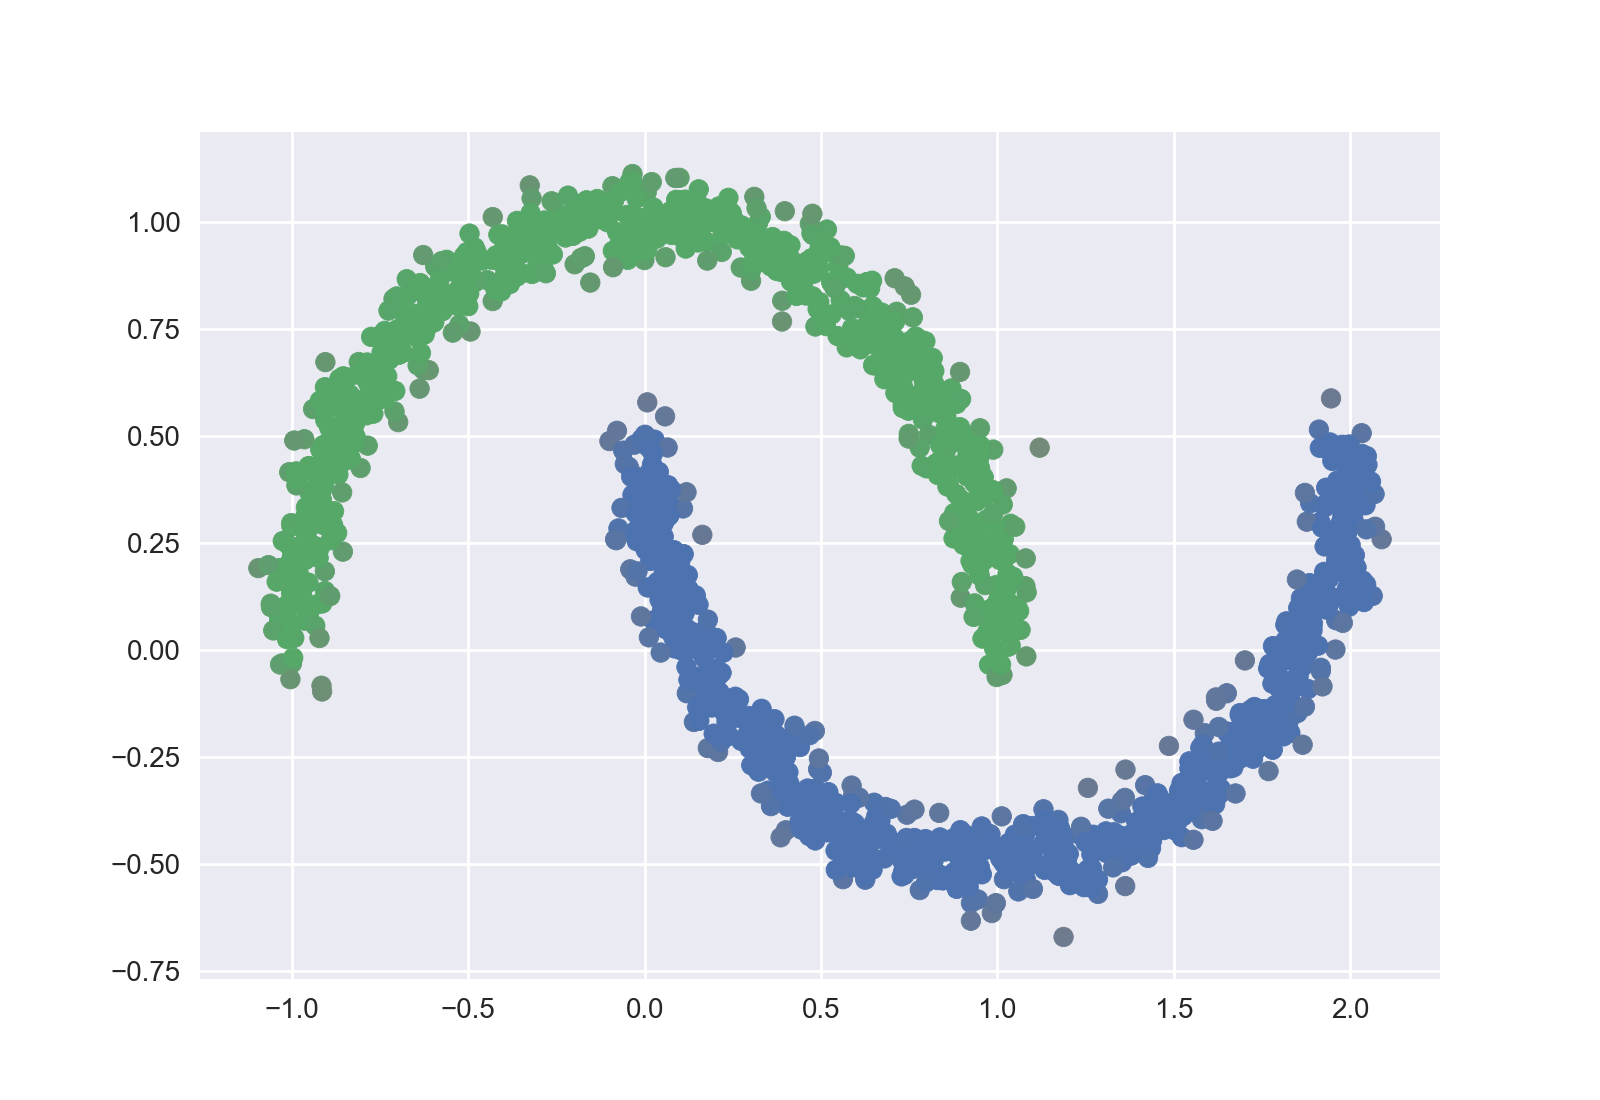
\includegraphics[width=\linewidth]{m_figure_2.png}
			\caption{}
		\end{subfigure}
		\caption{Clusters of moons}
	\end{figure}
%\end{comment}
	
	\newpage
	
	For high dimensional data, we test our algorithm on UCI datasets and check the cover rate of each dataset.
	
	\begin{table}[t]
		\caption{Cover rate on different UCI datasets}
		\label{sample-table}
		\centering
		\begin{tabular}{l  l  l  l  l }
			\toprule
			Datasets & wine & iris & yeast & red wine\\ \hline
			RSLFC & 49.3\% & 89.3\% & 31.1\% & 4.1\% \\ \hline
			K-means & 44.9\% & 66.6\% & 20.3\% & 3.2\%  \\ \hline
			DBSCAN & 0.0\% & 25.1\% & 2.6\% & 0.0\%  \\ \hline
		\end{tabular}
	\end{table}
	
	\begin{center}
		
	\end{center}
	
	\begin{figure}[h!]
		\centering
		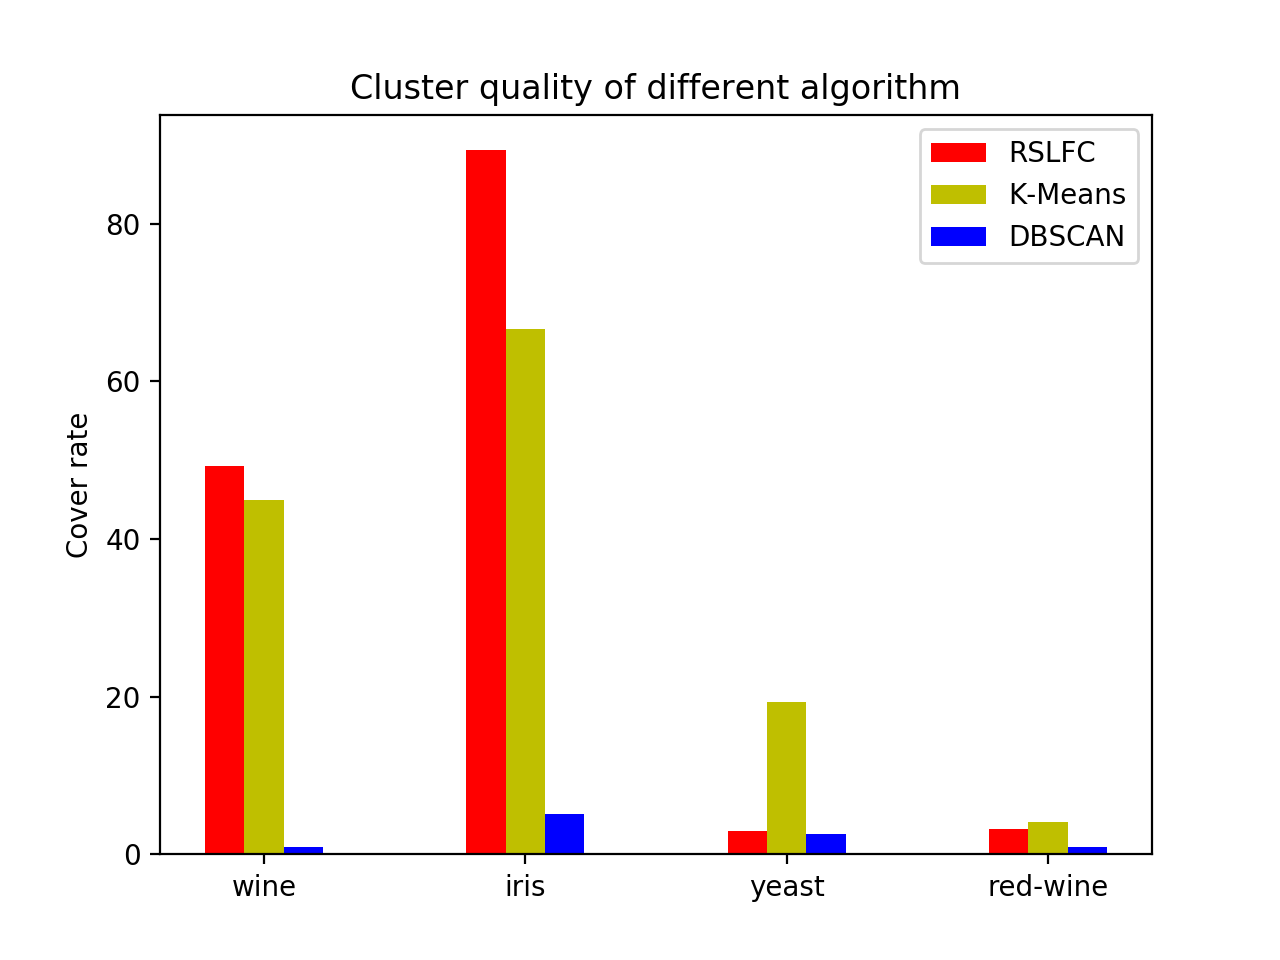
\includegraphics[scale=0.8]{hist1.png}
		\caption{Cover rates of RSLFC, K-Means, and DBSCAN}
	\end{figure}
	
\section*{References}

\small

[1] Campello, R. J., Moulavi, D., \& Sander, J. (2013). Density-based clustering based on hierarchical density estimates. In \emph{Pacific-asia conference on knowl- edge discovery and data mining} (pp. 160–172).

[2] Chaudhuri, K., \& Dasgupta, S. (2010). Rates of convergence for the cluster tree. In Advances in \emph{neural information processing systems} (pp. 343–351).

[3] McInnes, L., Healy, J., \& Astels, S. (2017, mar). hdbscan: Hierarchical density based clustering. \emph{The Journal of Open Source Software}, 2(11).
	
	
\end{document}
